\documentclass[conf]{new-aiaa}
\usepackage[utf8]{inputenc}

\usepackage{subcaption}
\usepackage{placeins}
\usepackage{cleveref}
\usepackage{graphicx}
\usepackage{amsmath}
\usepackage[version=4]{mhchem}
\usepackage[per-mode=symbol,separate-uncertainty = true,multi-part-units=single]{siunitx}
\usepackage{longtable,tabularx}
\setlength\LTleft{0pt} 
\usepackage{color}
\usepackage{epstopdf}
\usepackage{makecell}
\usepackage{url}
\usepackage{multirow}
\usepackage{float}
\usepackage[normalem]{ulem}

\usepackage{hyperref}

\sisetup{group-separator = {,}}

\graphicspath{{Figures/}}

\Crefname{equation}{Eq.}{Eqs.}
\Crefname{figure}{Fig.}{Figs.}

\DeclareSIUnit\inch{in}
\DeclareSIUnit\foot{ft}
\DeclareSIUnit\year{yr}
\DeclareSIUnit\kts{kts}
\DeclareSIUnit\poundforce{lbf}
\DeclareSIUnit\pixel{px}

\begin{document}

\begin{titlepage}

	\centering
	\vspace*{\fill}
	\rule{\textwidth}{0.4pt}
	\textsc{\huge Flight Test Report \\}
	\textsc{\huge Flight Test 04 (Aircraft Performance) \\}
	\bigskip
	\textsc{\large Date Submitted: May 11, 2020\\}
	\bigskip
	{\large Prepared by: \textsc{\huge Team Ramrod}\\}
	{(Shawn M. Herrington, Paul Klappa and Cody Smith)}	
	\rule{\textwidth}{0.4pt}
	
	\vspace*{\fill}	
	
	\begin{figure}[hbt!]
		\centering
		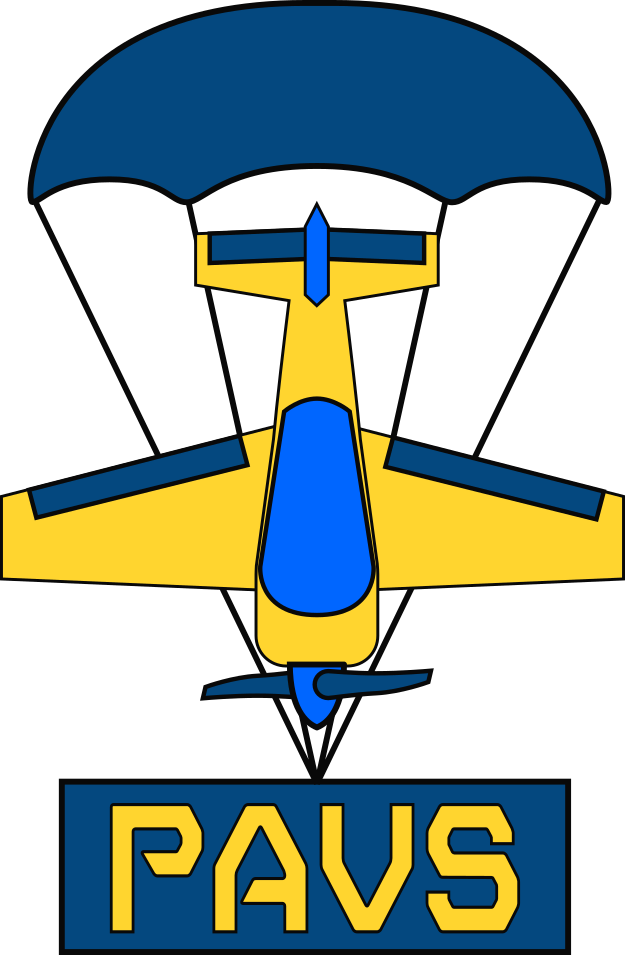
\includegraphics[height=1.75in]{PAVSLogo_BlackOutline.png}
		\label{PAVSLOGO}
	\end{figure}	
		
\end{titlepage}

\section{Introduction}

Assessing the flight performance characteristics of an aircraft is important when considering the aircraft capabilities. This test campaign focused on the assessment of the Piper Warrior II PA-28 and the Thorp T-18 – N249R series aircrafts while performing the level flight, climb, descent, takeoff, and landing maneuvers. Each maneuver has a characteristic airspeed that was recorded during the respective flight card maneuvers which will be discussed in more detail. 

\subsection{Test Objectives}

Level power required is determined during the level acceleration maneuver. During this maneuver, the flaps are set to~\SI{0}{\degree}~and throttle is steadily reduced until the flight speed achieves the stall speed. Once this state is achieved, the throttle is increased to full in order to allow the aircraft to stabilize at a maximum speed. The level power is found by taking aircraft measurements of fuel quantity and flow rate.

The climb rate is found from conducting the steady climb maneuver. During this maneuver, the aircraft trim is set to a desired airspeed with throttle set to full. The climb goes through~\SI{4000}{\foot} MSL or until~\SI{3}{\minute}. 

The descent rate is found by performing the steady descent maneuver. Throttle is set to idle during this maneuver as the descent goes through~\SI{2500}{\foot} MSL or for~\SI{3}{\minute}. This maneuver assumes the aircraft is close to level.

The takeoff distance is found during the short-field takeoff maneuver. The known aircraft starting point and the point of takeoff is the desired distance. The point where the aircraft takes off is the moment where the brakes are released and the aircraft achieves acceleration (point where nose wheel contact is lost with the ground). 

Landing distance was determined during the short-field landing maneuver. The distance is the displacement of the point of nose wheel contact with the ground and the complete stop position on the runway. The aircraft touchdown is within~\SI{100}{\foot}~of the runway numbers in order to achieve comparable landing repetitions.

\subsection{Team Ramrod}

Team Ramrod was established in 2019 with the goal of dethroning Tech N9ne as the most famous hip-hop act from Kansas City. Originally conceived as a foursome, the group was reduced to their current lineup after MC Tim Layman left the group due to creative differences. Following the success of their double platinum eponymous debut album, Team Ramrod shocked the world by walking away from their lucrative careers in the music industry in order to pursue advanced degrees in Mechanical Engineering.

\subsubsection{Shawn Herrington}

Shawn Herrington was born in Kansas City but he's a Florida man at heart. Shawn has rarely met a swear word he didn't immediately take a liking to. Shawn's number one skill is knowing the exact moment when someone has left the room so he can start talking about them behind their back. Often stirred into a furious rage over the most mundane things, Shawn can be made to put on an entertaining demonstration of overreaction just by asking him simple questions such as ``How are you doing today?'' or ``Did you get that email about the assignment?''.

\begin{figure}[hbt!]
	\centering
	
\includegraphics[height=1.5in]{ShawnExotic2.jpg}
	\label{PAVSLOGO}
	\caption{Discount Hulk Hogan}
\end{figure}

During flight tests, Shawn contributes as little as possible.  He earned the dubious distinction of being the only ``pilot'' (used loosely here) to successfully crash the notoriously milquetoast Cessna 172 in two out of three CG configurations. Shawn's hobbies include eating Cheetos Puffs\textsuperscript{\textregistered} with a fork (to avoid getting dusty orange fingers) and telling boring stories about his dog.  Annoyingly, Shawn has been known to refer to people, even people he's not related to as ``brother''.

\subsubsection{Paul Klappa}

Paul ``The Klapp'' Klappa is originally from great frozen tundra of the remote northern state of Minnesota. In addition to understanding the sport of hockey, Paul is distinguished by the way he pronounces ``bag'', ``rag'', etc. Despite his prolific professional wrestling career, Paul never let fame go to his head and even returns to Minnesota from time to time to participate in the regular ice fishing competitions held at any of of the states' famous \num{10000} lakes.

\begin{figure}[hbt!]
	\centering
	
\includegraphics[height=1.5in]{KlappIsCookin2.jpg}
	\label{PAVSLOGO}
	\caption{Can you smell what the Klapp is cookin'?!}
\end{figure}	

As the youngest and most charismatic member of \emph{Team Ramrod} Paul plays public relations manager for the team. Paul's main contributions to the team are making sure he is holding the correct brand of energy drink during press conferences to keep up that sweet sponsorship money. When he is not serving as test engineer, or repeatedly saying ``proceed'' awkwardly into the headset microphone Paul enjoys pumping some iron, hitting up the vending machine, and wearing sweatpants.

\subsubsection{Cody Smith}

Cody Smith hails from the greater metropolitan Kansas City area. Born and bred in the~\num{816} Cody represented his hood all over the world as crew chief for the world famous United States Air Force (USAF) B52 aerobatic demonstration team. Now living the calm civilian life, Cody scratches the thrill-seeker itch by hand-launching foam airplanes at great risk to life and limb. Ever courageous in the face of unspeakable danger, Cody answers questions like ''Dude, did you see how close that propeller was to your arm?'' with a simple shrug; just another routine day for this former USAF Airman.

\begin{figure}[hbt!]
	\centering
	
\includegraphics[height=1.5in]{CodyCena.jpg}
	\label{PAVSLOGO}
	\caption{Your time is up, my time is now!}
\end{figure}

Cody's role on \emph{Team Ramrod} is fashion consultant. Always dressed for the occasion, Cody is an expert on flight test engineering attire including cargo shorts and baseball caps. Due to his extensive experience working on real airplanes, Cody is always designated as the crew chief even when no crew chief is needed. When he's not pleading the case against Billy Joel to  his younger brother Simeon, Cody spends his free time watching his wife do squats and searching for that missing bag of trail-mix.


\section{Background}

\subsection{Level Flight Performance versus Power Required}

There are four forces on aircraft during flight. These forces are lift, weight, thrust, and drag. Lift acts perpendicular to the velocity. Drag acts parallel and opposite to velocity. Weight acts downward in the inertial reference frame. Finally, the thrust acts longitudinally in the body reference frame. The level flight performance in steady conditions relies on lift which is characterized by the following equations:

\begin{equation} \label{eq1}
\ L = W - T\sin(\theta_T)
\end{equation}

\begin{equation} \label{eq2}
\ D = T\cos(\theta_T)
\end{equation}

L is indicative of lift force, W is the weight, T is the thrust, and~$\theta_T$~is the angle of thrust. The drag force is produced as a by-product of lift and velocity. Aircrafts sustain flight by generating thrust to oppose drag. In order for the aircraft to achieve level flight performance, the following equations must be true:

\begin{equation} \label{eq3}
\ D_p = 1/2 \rho v^2 C_{D_p}
\end{equation}

\begin{equation} \label{eq4}
\ D_i = \frac{L^2}{1/2 \rho v^2 s \pi AR e}
\end{equation}

$D_{p}$~is the parasitic drag due to speed whereas~$D_{i}$~is the induced drag due to lift. ~$AR$~is the aspect ratio,~$e$~is the Oswald efficiency factor, and~$C_{D}$~is the drag coefficient.~$D_{p}$~will vary with~$v^{2}$~which is important to remember since increasing velocity will increase by the square of the velocity.~$D_{i}$~will vary with~$\frac{1}{v^2}$~which means induced drag decreases with increasing velocity.

The power required equation is based on force multiplied by the velocity. However, the power equation can be expanded into the following forms. It is important to note that power needs to be multiplied by about eight in order to achieve a velocity twice as fast.~$s$~represents the referenced frontal area of the aircraft (this reference can change depending on the geometry of the aircraft). The following equations show the substitutions required to yield the required power,~\textit{P}, equation.

\begin{equation} \label{eq5}
\ P = Dv
\end{equation}

\begin{equation} \label{eq6}
\ P = 1/2 \rho v^2 C_{D_p} s v
\end{equation}

\begin{equation} \label{eq7}
\ P = C_D s (1/2 \rho v^3)
\end{equation}

\begin{equation} \label{eq8}
\ D_p = 1/2 \rho v^2 C_{D_p} s
\end{equation}

\begin{equation} \label{eq9}
\ P = f (v^3)
\end{equation}

\subsection{Excess Power and Climbing Flight}
The climb performance of the aircraft follows the rate of climb equation where $\gamma$ is indicative of the flight path and not the propeller:

\begin{equation} \label{eq10}
\ R.O.C. = \frac{dH}{dt} = v \sin(\gamma)
\end{equation}

Climbing flight relies on the force from the time rate of change of height. Thrust horsepower excess, $THP_{excess}$, is another variable that is dependent on the height time rate of change and aircraft weight, $W$. 

\begin{equation} \label{eq11}
\ THP_{excess} = W \frac{dH}{dt}
\end{equation}

There is a power required curve for flight at specific velocities and a power available curve. The power required by the system is typically under the available power curve, and the excess thrust is the difference between the two curves. However, there is a point (crossover point) where more power is required to climb at a higher velocity than what is currently available for an aircraft. Thus, knowing the best angle of climb is important. The best angle of climb occurs right before the peak of the rate of climb on the R.O.C. plot versus velocity. There is also a best angle where the aircraft is flown steeply as possible to avoid low altitude obstacles. Once the obstacles are cleared, the best rate of climb is used. 

\subsection{Gliding Flight}

Gliding refers to the steady-state flight condition in which an aircraft is maneuvering unpowered through the air without thrust. In the case of an airplane, gliding performance is measured when the aircraft's engine is completely unpowered. In previous sections, the aircraft was assumed to be at level flight. In the case of a glide, the aircraft is incapable of maintaining level flight and must descend at a particular angle. As airspeed increases, the aircraft must pitch down in order to allow a larger component of weight to counteract the drag.

An analysis can be peformed on an aircraft's glide performance through the use of a glide polar plot. A glide polar uses an inverted axes system with \(\dot{h}\), the sink rate, on the y-axis and the airspeed \(V\) on the x-axis. The glide polar plot is essentially a plot of how fast the aircraft descends as a function of different airspeeds. The glide polar can be used to determine glide characteristics like minimum descent speed which is the speed at which an aircraft should fly in order to stay airborne as long as possible. A tangent angle can be applied to the curve to determine the best angle of glide. The best angle of glide refers to the angle at which the aircraft must fly in order to fly the farthest distance possible. A glide polar provides insight into both aircraft performance and proper emergency procedures. The glide polar provides a pilot with useful information to extract the maximum performance from the aircraft in emergency conditions. 

\subsection{Takeoff and Landing Performance}


The forces required during takeoff can be described in \Cref{TO}. This equation is simply a Newton's 2nd Law representation of the sum of forces during takeoff equal to the mass times acceleration. The sum of forces can be broken down into thrust minus the aircraft's total resistance to liftoff. The total resistance during takeoff is displayed in \Cref{resistance} which is just the same of the aircraft's drag with it's rolling resistance while on the ground.

\begin{equation} \label{TO}
\ T - [D + \mu (W-L)] = \dfrac{w}{g}a
\end{equation}

where: 
\begin{tabbing}
\phantom{$D_{n50}\ $}\= \kill
\indent $T$\> \indent = Thrust\\
\indent $D$\> \indent = Aerodynamic Drag\\
\indent $\mu$\> \indent = Rolling Friction Coefficient\\
\indent $W$\> \indent = Weight on Wheels\\
\indent $L$\> \indent = Lift\\
\indent $g$\> \indent = Gravitational Constant\\
\end{tabbing}\

\begin{equation} \label{resistance}
\ R = [D + \mu(W-L)]
\end{equation}

Eventually, once the aircraft has left the ground, the weight on the aircraft's wheels goes to zero and the total resistance on the aircraft is only equal to the drag. The total resistance on the aircraft can be expanded further in equation \Cref{expandresistance} which is a complex breakdown of the drag force.

\begin{equation} \label{expandresistance}
\ R = (C_{D_P} + \dfrac{C_{L}^2}{\pi ARe})qS + \mu(W-C_LqS)
\end{equation}

where: 
\begin{tabbing}
\phantom{$D_{n50}\ $}\= \kill
\indent $C_{D_P}$\> \indent = Parasitic Drag\\
\indent $C_L$\> \indent = Coefficient of Lift\\
\indent $A$\> \indent = Aspect Ratio \\
\indent $e$\> \indent = Efficiency Factor\\

\end{tabbing}\

The aspect ratio is the square of the aircraft's wingspan divided by the wing area. The efficiency factor e is equal to 1.0 for an elliptical distribution and is generally some value less than 1.0 for any other lift distribution \cite{NASA}. 

During a takeoff maneuver, \Cref{thrustexcess} can be viewed from a work perspective which is the work that is performed during a takeoff roll. This perspective is shown in \Cref{workperspective}. Here \(S_{gTO}\) refers to the distance the aircraft needs to roll on the ground before takeoff. Further rearranging \Cref{workperspective} leads to \Cref{groundrolldistance} which is used to solve for the ground roll distance.

\begin{equation} \label{thrustexcess}
T_{excess} = T_{net} - R
\end{equation}

\begin{equation} \label{workperspective}
(T_{net} - R)S_{gTO} = (\dfrac{W}{2g})V_{TO}^2
\end{equation}

\Cref{groundrolldistance} shows that ground roll distance changes as a function of net thrust and weight. If the aircraft is given more thrust the ground roll distance is decreased. Likewise, the ground roll takeoff distance has a 1:1 change when affecting weight. That is, if you double weight you double the distance required for the aircraft to takeoff. \(V_{TO}\), the takeoff velocity, can also be changed in order to compensate for increased weights or increased resistances. That is, the heavier an aircraft is or the more resistance during takeoff, the faster the aircraft must go to takeoff in the same rolling distance. 

\begin{equation} \label{groundrolldistance}
S_{gTO} = \dfrac{W}{g(T_{net}-R_{nom})}(\dfrac{V_{TO}^2}{2})
\end{equation}

\section{Test Procedure}

\subsection{Overview of Processes and Equipment}

\subsubsection{Process}

For each flight card there was a clearly defined checklist / procedure as well as one checklist for the pre-flight of the aircraft. The pre-flight checklist included standard airworthiness checks of the aircraft, instrumentation checks, passenger readiness checks, Go/No-Go Poll, etc. Each maneuver had specific checklist items relative to that maneuver. 

\subsubsection{Equipment}

For the first day of flight testing on April 23, the provided aircraft was a rental Piper P28-A Warrior II - N6394C. The Piper was piloted by Dr. Abdulrahim for all three flights of the day. On April 28, for the second day of flight testing, both the Piper P28-A and a Dr. Field's Thorpe T-18-N2494 were flown. The third test flight day  Additional instrumentation added to each aircraft for flight testing was the Pixhawk 2.1, Here2 GPS, and a telemetry radio inside the cabin. Mounted on the outside of the wing was a PixRacer, mRo Gps, pitot tube, and pressure sensor. 

\subsection{Narrative of the test process and sequence}

Following the order of the flight cards, the flight tests were conducted in a logical sequential order. The purpose of this test was to identify the aircraft performance characteristics in level flight, climb, descent, takeoff, and landing as well as identify characteristics including:

\begin{itemize}
\item Best endurance
\item Best range
\item Best climb rate
\item Best climb angle
\item Minimum sink rate
\item Best glide angle
\end{itemize}

\medskip
Other Maximum performance measurements include:

\begin{itemize}
\item Takeoff distance
\item 50 ft obstacle clearance
\item Landing Distance
\item Landing a 50 ft obstacle
\end{itemize}

\medskip 

Once the aircraft was in the air, and all personnel were ready to to begin the flight test, a generalized procedure for each flight card was followed. 

\medskip

\begin{enumerate}

	\item Test Director announces the start of the the test card  and conducts Go/No-Go Poll
	\item Test Director announces the specific test conditions
	\item Pilot maneuvers the aircraft into specific test condition
	\item Flight Test Engineer makes measurement call outs and records data
	\item Test Director reports maneuver or test card complete and proceeds to next flight card or end of test
\end{enumerate}

\medskip Once all flight cards were complete, after the conclusion of the short-field landing, the the test was concluded and the aircraft was brought back to the hangar to prepare for the next test.

\subsection{Flight Card}
\subsubsection{Maneuvers}
Based on the flight cards, there were several in-flight maneuvers planned for the experiment. Those maneuvers included:
\medskip
\begin{itemize}
\item \textbf{Short-Field Takeoff} for maximum performance takeoff and obstacle clearnace performance
\item \textbf{Level Acceleration} for level flight power required assessment
\item \textbf{Steady Climbs} for climb performance assessment
\item \textbf{Steady Descents} for descent assessment
\item \textbf{Short-Field Landing} for maximum performance obstacle clearance and landing performance
\end{itemize}

\medskip


The short-field takeoff is a maneuver that is performed when an aircraft is required to takeoff where runway length is limited. According to the flight cards, a short field takeoff is performed by lining up the aircraft with a known point on the runway, extending the flaps to 25 degrees, applying maximum brake pressure and increasing the throttle to full. The brakes are then released allowing the aircraft to accelerate to 52 KIAS until the aircraft was 50 AGL. The aircraft is then accelerated to 79 KIAS at which point then flaps are to be slowly retracted allowing the aircraft to climb until 1000 AGL. Assesment criteria includes:

\medskip

\begin{itemize}
\item Throttle reaches maximum before brakes released
\item Airspeed at rotation with +5/-2 KIAS of 52 KIAS
\item Initial climb speed remains within +5/-2 KIAS of 52 KIAS
\item Final climb speed remains within +/-5 KIAS of 79 KIAS
\item Steady climb maintained until above 1000ft AGL
\end{itemize}

\medskip

A level acceleration maneuver is when the aircraft attempts to stay at a fixed altitude and then fly from the minimum speed to the maximum speed and back down slowly. By doing this with the correct instrumentation a power required curve can be developed which provides, at a particular altitude, what power is required at each particular airspeed. The procedure for the level acceleration maneuver is to climb to 3000 ft MSL and set flaps to 0 degrees. At that point, throttle is reduced steadily until the aircraft maintains altitude at its stall speed. The throttle is then increased to full allowing the aircraft to stabilize at its maximum speed. The power is then reduced in 10\% increments. For each throttle increment, the airspeed is required to be stabilized whereby data is recorded until the aircraft once again reaches its stall speed. Assesment criteria includes: 

\medskip

\begin{itemize}
\item Airspeed stabilizes at each test point
\item Altitude remains within 100 feet throughout the maneuver
\item Bank angle remains within 5 degrees of level
\end{itemize}

\medskip

An aircraft's climb performance varies tremendously depending on the airspeed chosen. For each groups flight a steady climb maneuver was performed in order to obtain multiple assessments of climb rate at different airspeeds. A steady climb maneuver is performed by climbing the aircraft to 2500 ft MSL and setting the flaps to 0 degrees. At that point, the aircraft is trimmed to the desired airspeed and throttle is set to full. The aircraft is then positioned to climb through 4000 ft MSL or for 3 minutes. This maneuver enables the building of the climb power curve to determine the maximum angle and most efficient climb rate. Assessment criteria for the steady climb is:

\medskip
\begin{itemize}
\item Airspeed remains within 5 knots of desired airspeed
\item Climb speed remains within +/- 100 ft/min
\item Bank angle remains clear of clouds
\item Aircraft does not encounter moderate or higher turbulence
\end{itemize}

\medskip

Steady descents, in the case of powered aircraft, are of concern primarily in emergency situations. In the event of engine failure it is necessary to understand how to manage airspeed in order to achieve the greatest range the aircraft can provide. Again, this maneuver was performed with varying angles for each group. The steady descent maneuver is performed by climbing to 4000 ft MSL and setting the flaps to 0 degrees. The aircraft is then trimmed to the desired airspeed and throttle is set to idle. The aircraft then descends through 2500 ft MSL or for 3 minutes. Assement criteria for the steady descent maneuver is:

\medskip

\begin{itemize}
\item Airspeed remains within 5 knots of desired airspeed
\item Descent speed remains within +/- 100 ft/min
\item Bank angle remains within 5 degrees of level 
\item Aircraft remains clear of clouds
\item Aircraft does not encounter moderate or higher turbulence
\end{itemize}

\medskip

Short-field landing is a maneuver where the aircraft descend at the normal rate and but stops at a faster than normal speed. The short-field landing maneuver is performed by establishing a 3 degree glide path on final approach, trimming the airspeed to 63 KIAS and setting flaps to 40 degrees. Once the aircraft lands on the runway numbers, full brakes are applied after the nose wheel touches the ground until the aircraft comes to a complete stop. Assesment criteria for the short-field landing is:

\medskip

\begin{itemize}
\item Aircraft established on 3 degree glide path on final approach
\item Steady descent rate on final approach
\item Airspeed remains within +/- 5 KIAS of 63 KIAS  
\item Aircraft touches down within 100 feet of runway numbers
\item Aircraft comes to complete stop for 5 seconds on runway
\end{itemize}

\medskip


\subsubsection{Modifications to Aircraft}

Modifications to the aircraft N6394C include instrumenting a Pixhawk 2.1, Here2 GPS, and a telemetry radio inside the cabin. Additionally, a PixRacer, mRO GPS, pitot tube, and pressure sensor were mounted on the underside of the wing. Redundant sensors were used in order to ensure quality data for the performance assesment.

\subsubsection{Weather}

Since the test involves the use of an actual aircraft carrying personnel, it was important to keep track of weather more thoroughly than in prior tests. Weather and atmospheric conditions were logged for each flight card.


\subsubsection{Time}

Two separate times were recorded for the flight test: 'Test Time' and 'Flight Time'. The 'Test Time' encompasses the entirety of the test to include setup, pre-flight and post-flight procedures, and flight. The 'Flight Time' includes only the time spent in the air.

\subsubsection{Risk Assessment}

For this particular test, the risks involved were much more concerning than previous tests. Since the flight test includes the use of an actual physical aircraft and for many students being inexperienced in that field, the following risks were considered:

\medskip
\begin{itemize}
\item Risk of passenger discomfort or nausea during maneuvers
\item Risk of turbulence or high winds affecting flight performance
\item Risk of low visibility or poor weather affecting flight schedule
\end{itemize}

At any point throughout the test, if a passenger felt unresolvable discomfort for any reason, the passenger could simply say they were ready to land and the pilot would have landed. 

\subsection{Anomalies}

Two known anomalies occurred throughout the course of the flight tests. The first anomaly occurred when a bolt for the the required external instrumentation did not fit the rental aircraft. The attachment hardware had been previously tested on the Thorpe, but was incompatible for the rented Piper. Fortunately, someone at the airfield was able to help resolve the situation. The second anomaly that occurred was the  external instrumentation the RFD telemetry system was drawing excessive amounts of power essentially browning out the pixracer. To resolve the issue, the external instrumentation was run without telemetry because a backup power source was unavailable.   
\subsection{Flight Card}

As discussed in detail throughout the procedure, the flight cards were followed systematically throughout the flight test. An attached copy of the flight cards can be seen in the Appendix. 

\section{Test Results}

\begin{itemize}
	\item Show plots of level flight acceleration
	\item Show plots of climbs and descents
\end{itemize}

\subsection{Takeoff Performance}

The takeoff performance was found from the data using various indicator variables to determine two critical points the first being the instant the take-off roll began and the second being the moment the aircraft completed rotation and departed the runway. Various variables can be used in this endeavor and carefully studying video from on-board cameras would have been another method if the video had been provided. For most of the flight tests, three independent estimates of the moment the takeoff roll began were available from the following measurements: velocity, pitch rate and accelerometer.

For the velocity measurement, a point of near zero velocity was easily identified which was immediately followed by a period of steadily increasing velocity. The difficulty in determining the start of takeoff roll from the velocity measurement is two fold. Firstly, since this is a measurement via global positioning system (GPS) it may lag the true takeoff roll instant and this time lag can be variable depending on the current estimate of error in the GPS signal. Analysis of the GPS signal lag and error is outside the scope of this report. The second difficulty arises because the velocity is never truly measured as zero and since the aircraft did not dwell on the runway, it can be difficult to determine what the noise level is corresponding to ``approximately'' zero velocity.

The pitch rate is determined from a gyroscope sensor. The main difficulty with the pitch rate data is that it is noisy. In fact, what would be expected to an obvious change on takeoff rotation in the pitch rate is not visible above the noise floor of the data. It was necessary to use another estimate of the beginning of the takeoff roll instant when analyzing the pitch rate data because of the noise level. Once an approximate location was identified, the nearest maximum or minimum spike in the pitch rate (usually corresponding to spikes in the other angular rates as well) was identified as the instant of the start of the takeoff roll. This spike is most likely due to the pitching of the plane due to releasing the brakes or possibly the a rolling or yawing impulse due to the p-factor effect of the propeller.

The accelerometer measurement was used in a similar manner to the pitch rate measurement. Since this data can be very noisy, an approximate location was identified and then a local extremum was identified. This instant of this extreme point was then identified as the instant at which takeoff roll began.

Due to the uncertain nature of identifying takeoff roll beginning and end points, different sensors were used to identify different points of the flight test. Specifically the velocity and accelerometer measurements were only appropriate for identifying the beginning of the takeoff roll. While the pitch rate measurement was used to identify both the start and end of takeoff roll. Likewise, measurement of pitch angle and altitude were only useful in determining the instant of rotation (the end of takeoff roll) and are explained in more detail below.

The pitch angle was only useful in determining the end of the rotation, signifying the beginning of flight and the end of the takeoff roll. Frustratingly the pitch angle could not be used to identifying the beginning of the takeoff roll. This is likely due to two issues. The first issue is that the pitch angle is not perfectly zero while the plane in on the ground. Additionally, the pitch angle changes based on use of the brakes and the throttle position as well as with the movement of the occupants. The second problem with the pitch angle is that the small nose up attitude required for takeoff rotation means that the signal-to-noise ratio was low. Since this is not a flight test conducted with a high performance aircraft, the expected earth-shattering nose up pitch toward the sky does not occur and the relatively mild takeoff rotation is actually fairly difficult to identify (much less identifying the starting point of the roll).

The pitch rate measurement was used in a similar manner as before. The approximate location of the rotation point was idenfitfied from other data and then a local extremum was identified in the pitch rate measurements. The instant of this extremum was identified as the instant of the end of the takeoff roll.

The altitude can be used to idenfity the instant the aircraft left the ground (because the altitude began to increase). Fortunately, the altitude increase due to takeoff is large enough to provide a substantial signal-to-noise ratio making the instant easy to identify. Since altitude is provided barometrically, this data will not lag the actual data the way GPS altitude would. Altitude cannot be used to determine the start of the takeoff roll because the altitude is approximately constant while the aircraft is on the ground.

The average takeoff roll distance was computed by comparing data for all 4 repetitions of the experiment captures as part of Flight Test 04, Card 1, Instance 1. The individual estimates are presented in~\Cref{takeofftable} below.

\begin{table}[htp!]
\centering
\caption{takeoff Roll Estimates.}
\label{takeofftable}
\begin{tabular}{ c | c | c | c }
	\multicolumn{4}{c}{\textbf{Repetition Number}}										\\
	\textbf{1} & \textbf{2} & \textbf{3} & \textbf{4}									\\
	\hline
	\SI{1785}{\foot} & \SI{2169}{\foot} & \SI{2355}{\foot} & \SI{1868}{\foot}			\\
	\hline
	\hline
	\multicolumn{3}{c}{\textbf{Overall Average}} & \textbf{\SI[detect-weight=true]{2044}{\foot}}	\\
	\hline
\end{tabular}
\end{table}

An example of the plots used to identify the individual estimates for the beginning and end of the takeoff roll is provided in~\Cref{takeofftimeid}. A plot showing all of the beginning and end times on the distance measurement is shown in~\Cref{takeoffdistanceid}.

\begin{figure}[htp!]
\centering
	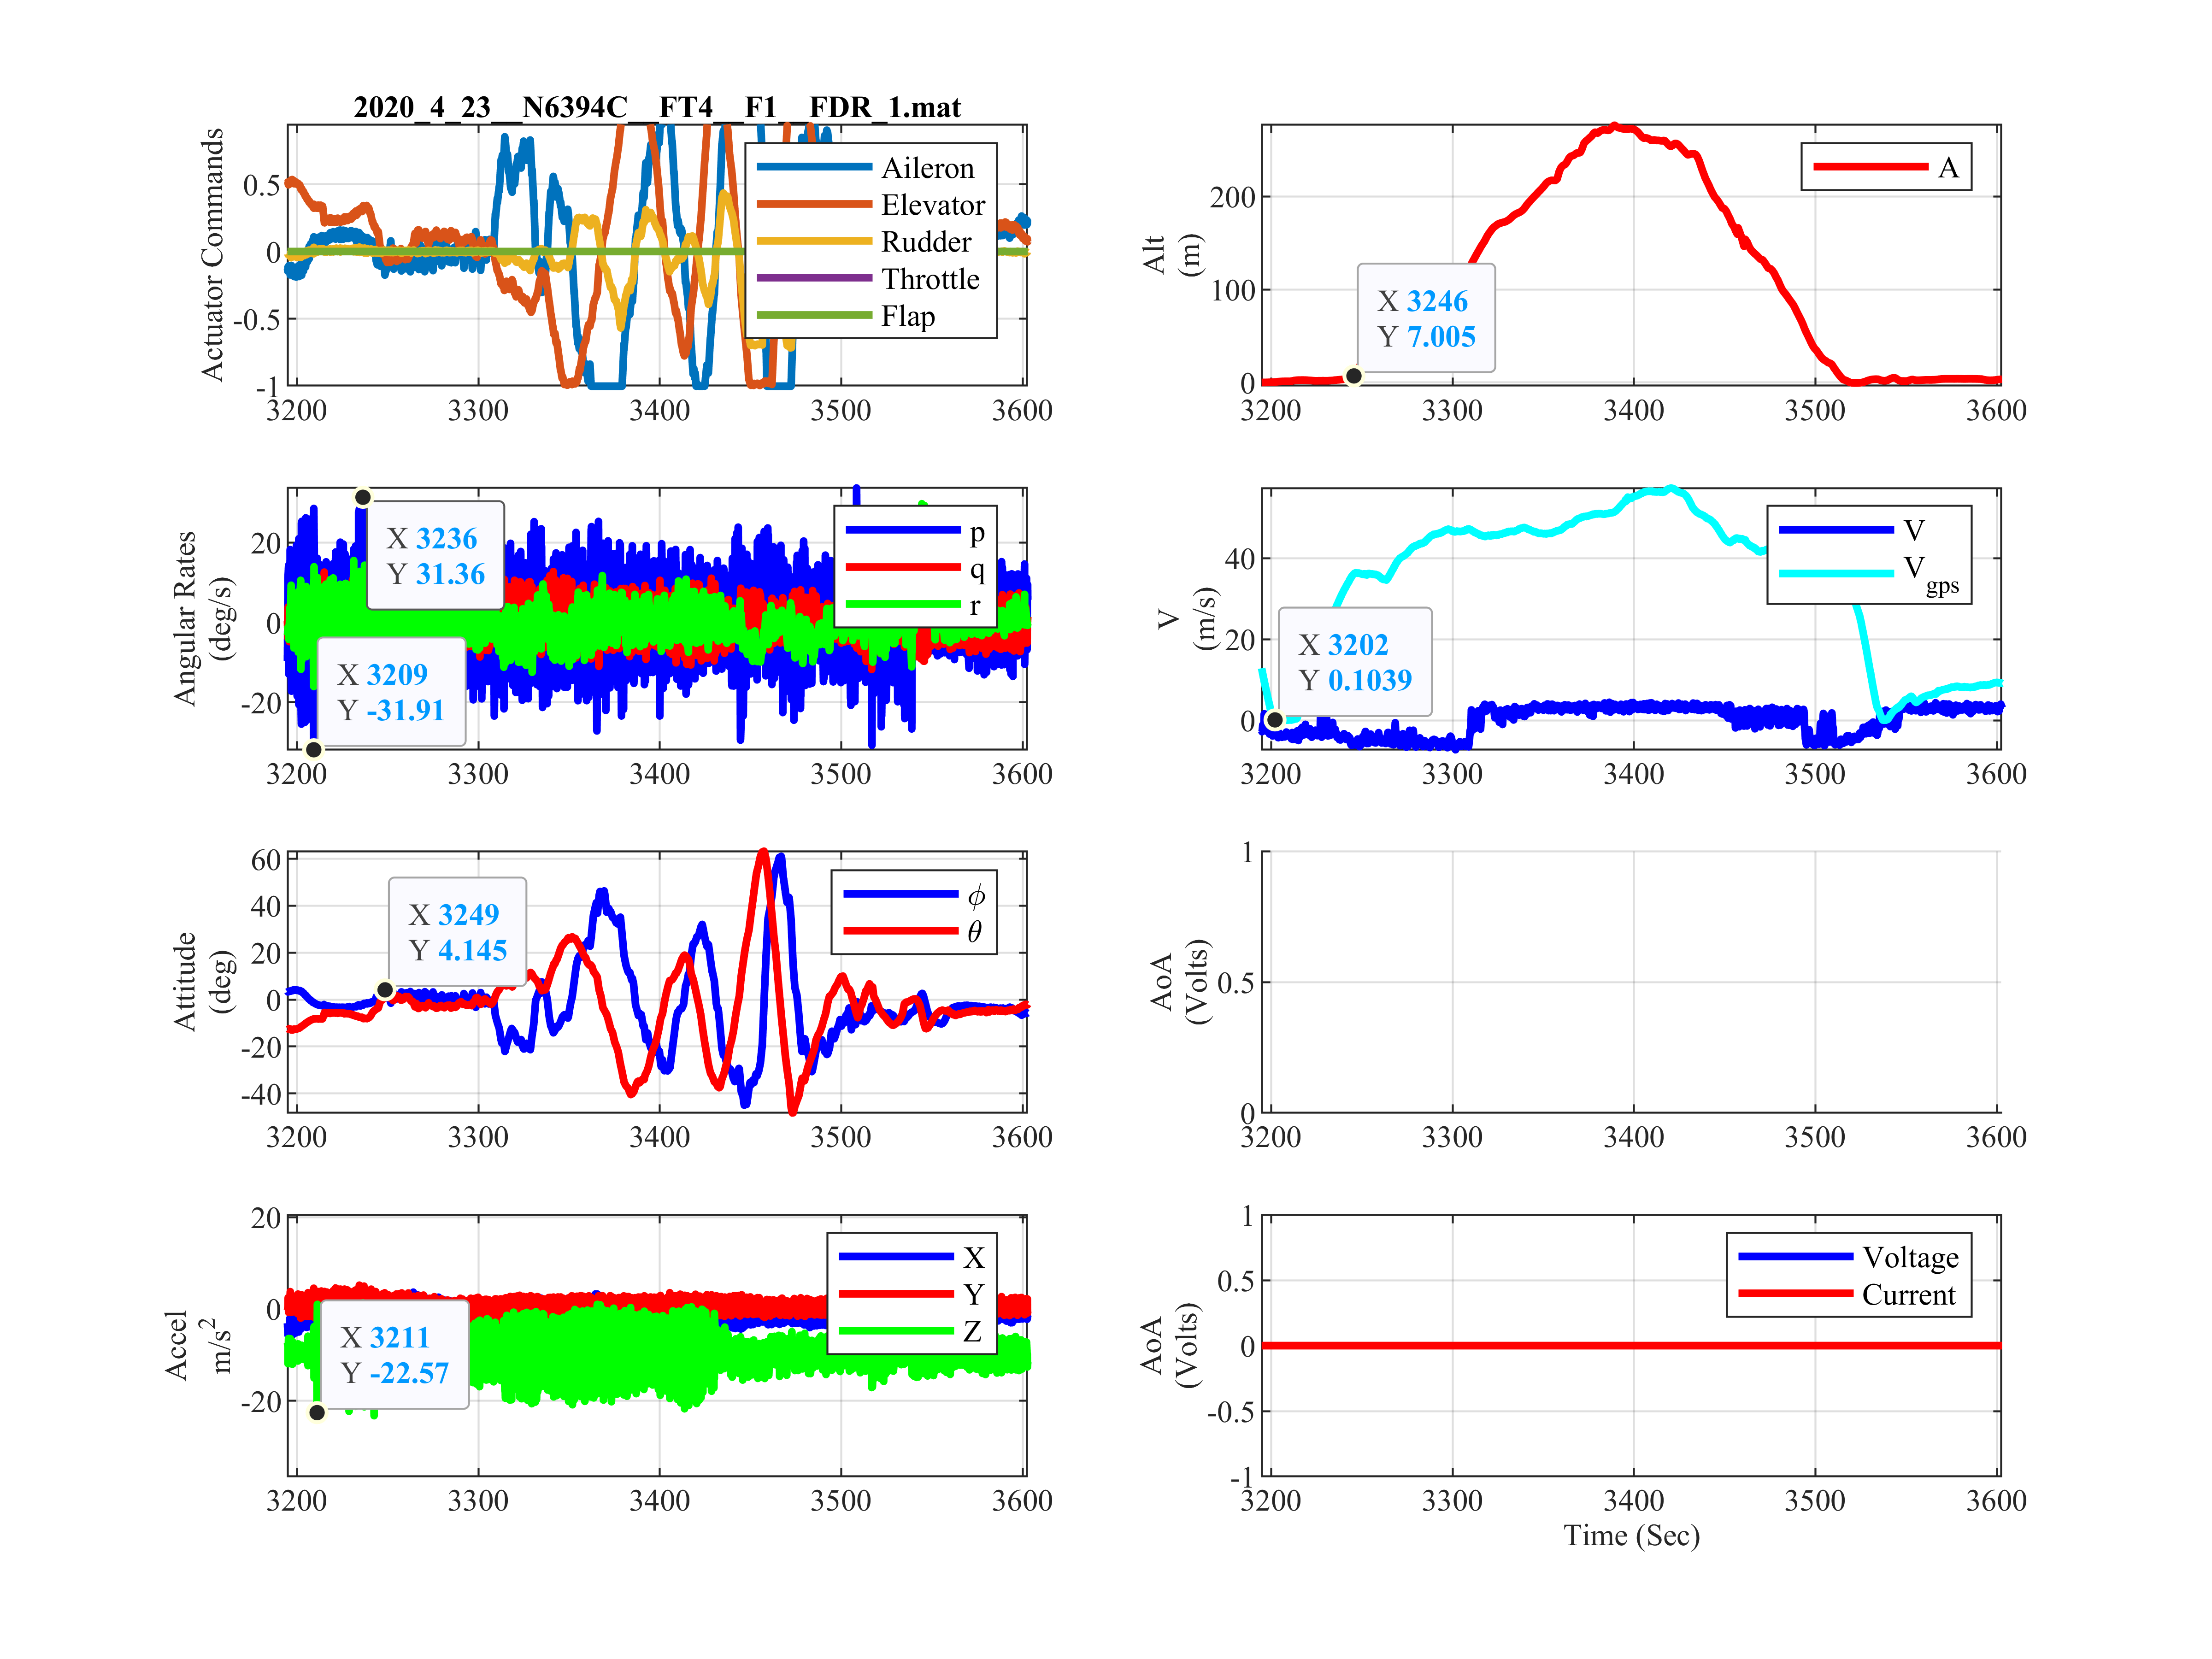
\includegraphics[height=4in]{TakeoffRollTimeID.png}
	\caption{Example of Identification of takeoff Roll Start and End Times.}
	\label{takeofftimeid}
\end{figure}

\begin{figure}[htp!]
\centering
	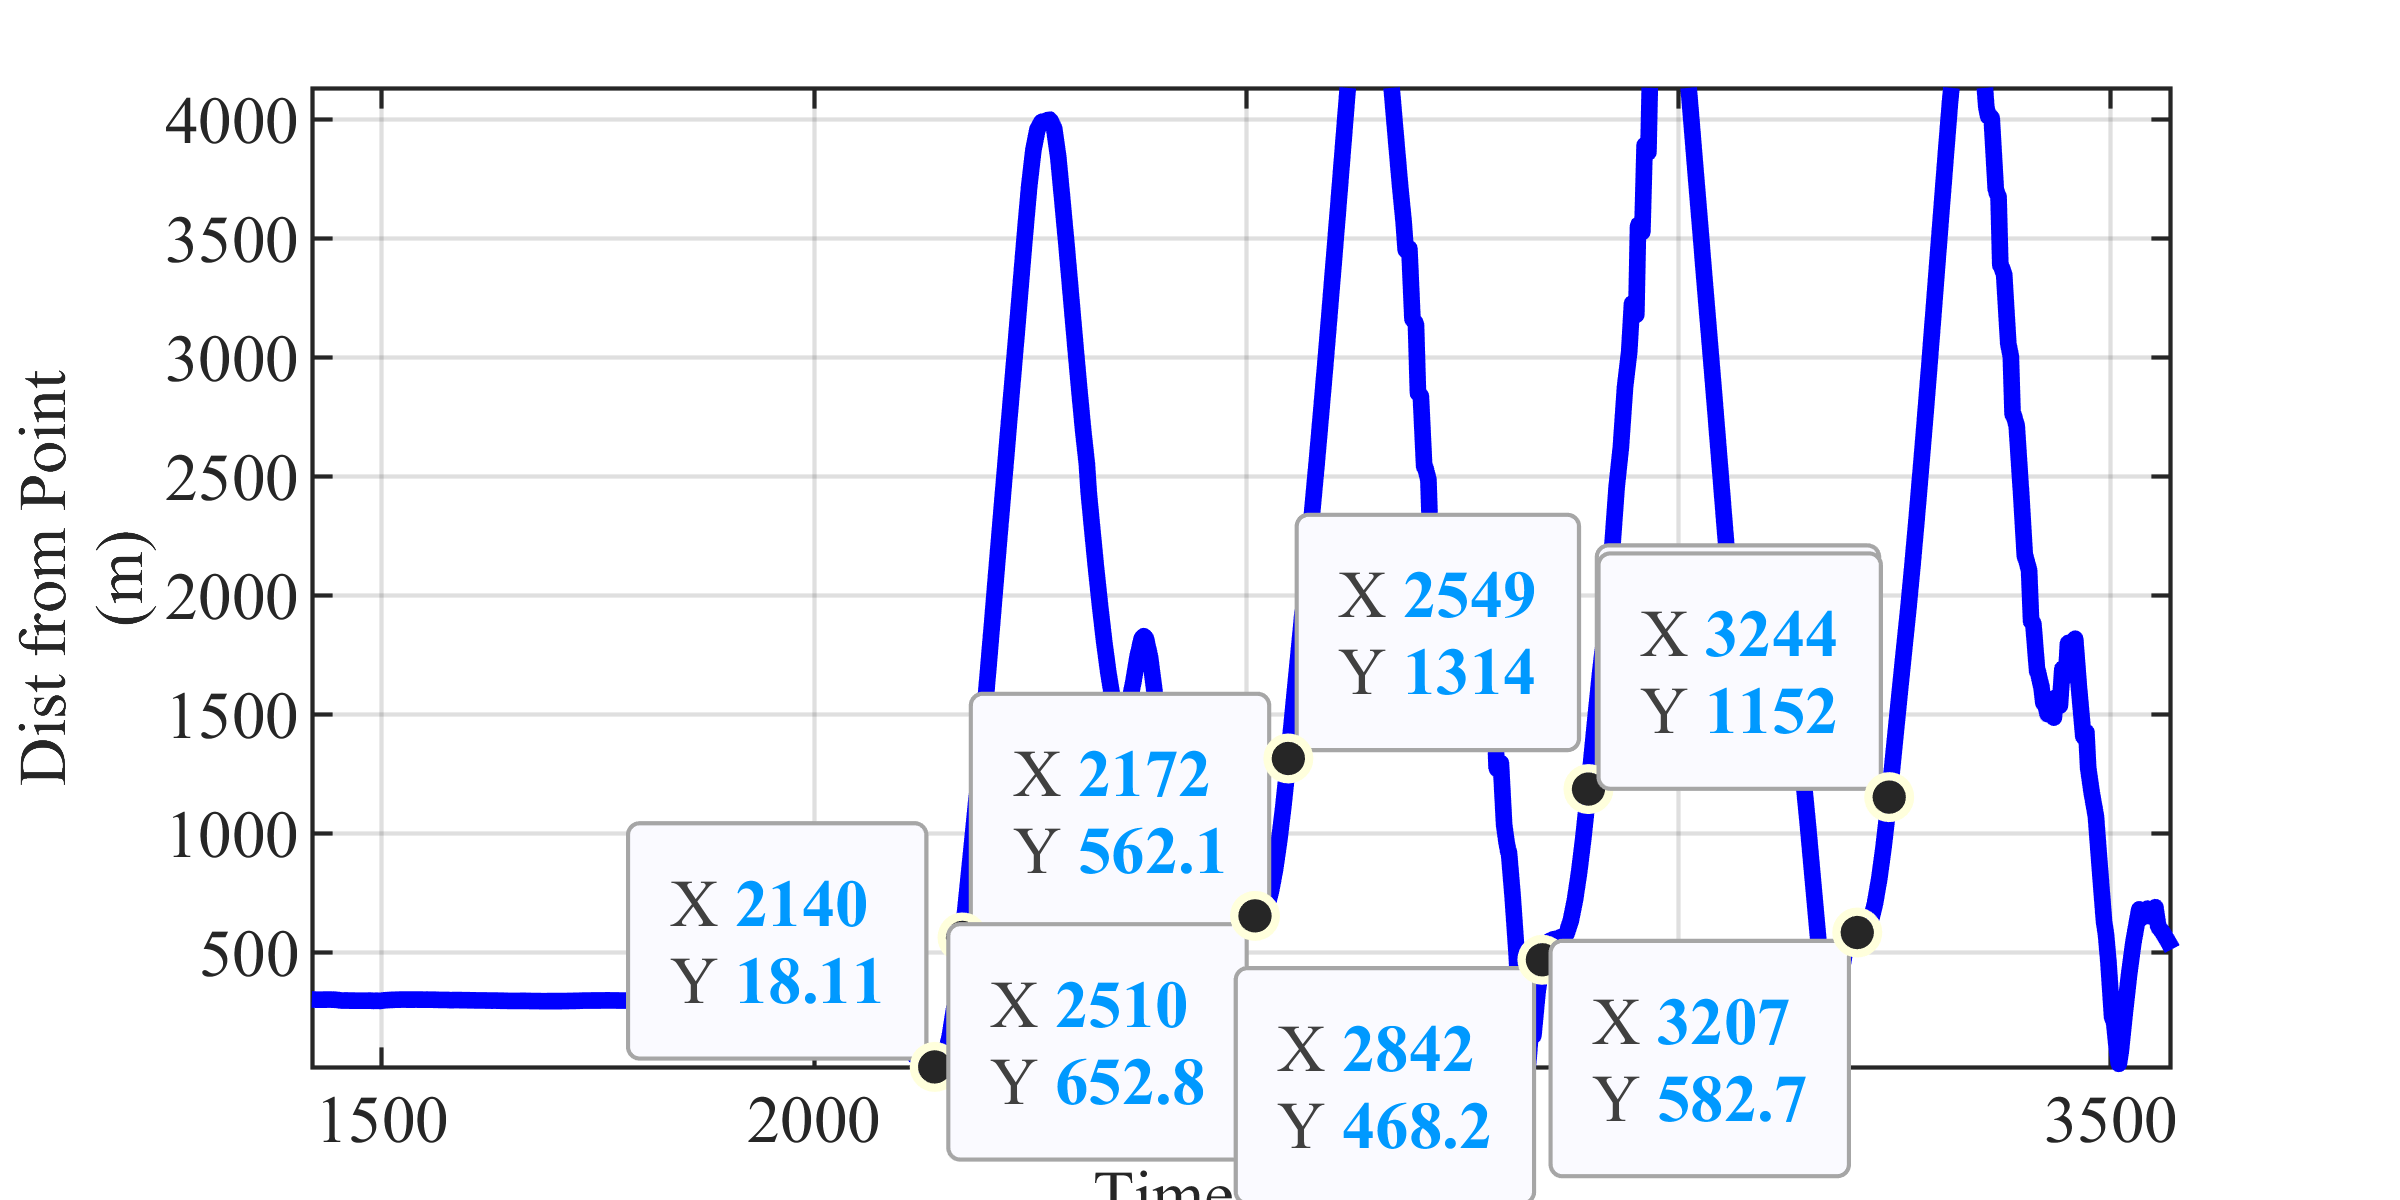
\includegraphics[height=1.5in]{TakeoffRollDistID.png}
	\caption{takeoff Roll Distance Identification using Previously Identified Time Instants.}
	\label{taekoffdistanceid}
\end{figure}

The pilot operating handbook (POH) for the aircraft used during this flight test puts the takeoff roll distance at around~\SI{2000}{\foot}. No information on the aircraft fuel load was given; although, another flight test was completed without refueling so the aircraft was not close to empty at the beginning of this test. Additionally, the aircraft was occupied by three passengers with an average estimated weight of~\SI{180}{\poundforce}. Assuming a basic empty weight of~\SI{1400}{\poundforce} along with about~\SI{100}{\poundforce} of fuel along with~\SI{100}{\poundforce} of additional equipment (I do not have the operating handbook for this particular aircraft but there was definitely additional equipment including a fire extinguisher, toolbox and upgraded avionics) gives an estimate for takeoff weight of~\SI{2140}{\poundforce}.

The identified takeoff roll of~\SI{2044}{\foot} is very close to the expected takeoff roll from the handbook of~\SI{2100}{\foot} (assuming altitude of~\SI{1000}{\foot} MSL and temperature of~\SI{15}{\celsius} according to the METAR for KMKC at the time of the flight test). This indicates that the takeoff test was conducted with adequately controlled conditioned since the test was able to recreate expected conditions. Additionally, it means that the pilot operating handbook is trustworthy (good news pilots!).

\subsection{Landing Performance}

For landing performance, a similar procedure to that used to find takeoff performance was used. In the case of landing performance, velocity, pitch angle and accelerometer measurements were available to determine the end of the landing roll. Only a single measurement, altitude, was available for identifying the touch down point. Ostensibly, the accelerometer, angular rate or the Euler angles should have indicated the instant of touch down. Practically, this was not possible. Reasons for this have been previously discussed in detail and include poor signal-to-noise ratio and the relatively mundane handling characteristics of the airplane in question. It might even be reasonable to hazard such a statement as the lack of appreciable impulse in any of the measurements during landing is a testament to the skill of the pilot.

\begin{table}[htp!]
\centering
\caption{Landing Roll Estimates.}
\label{takeofftable}
\begin{tabular}{ c | c | c | c }
	\multicolumn{4}{c}{\textbf{Repetition Number}}										\\
	\textbf{1} & \textbf{2} & \textbf{3} & \textbf{4}									\\
	\hline
	\SI{1358}{\foot} & \SI{1265}{\foot} & \SI{1026}{\foot} & \SI{1250}{\foot}			\\
	\hline
	\hline
	\multicolumn{3}{c}{\textbf{Overall Average}} & \textbf{\SI[detect-weight=true]{1225}{\foot}}	\\
	\hline
\end{tabular}
\end{table}

\begin{figure}[htp!]
\centering
	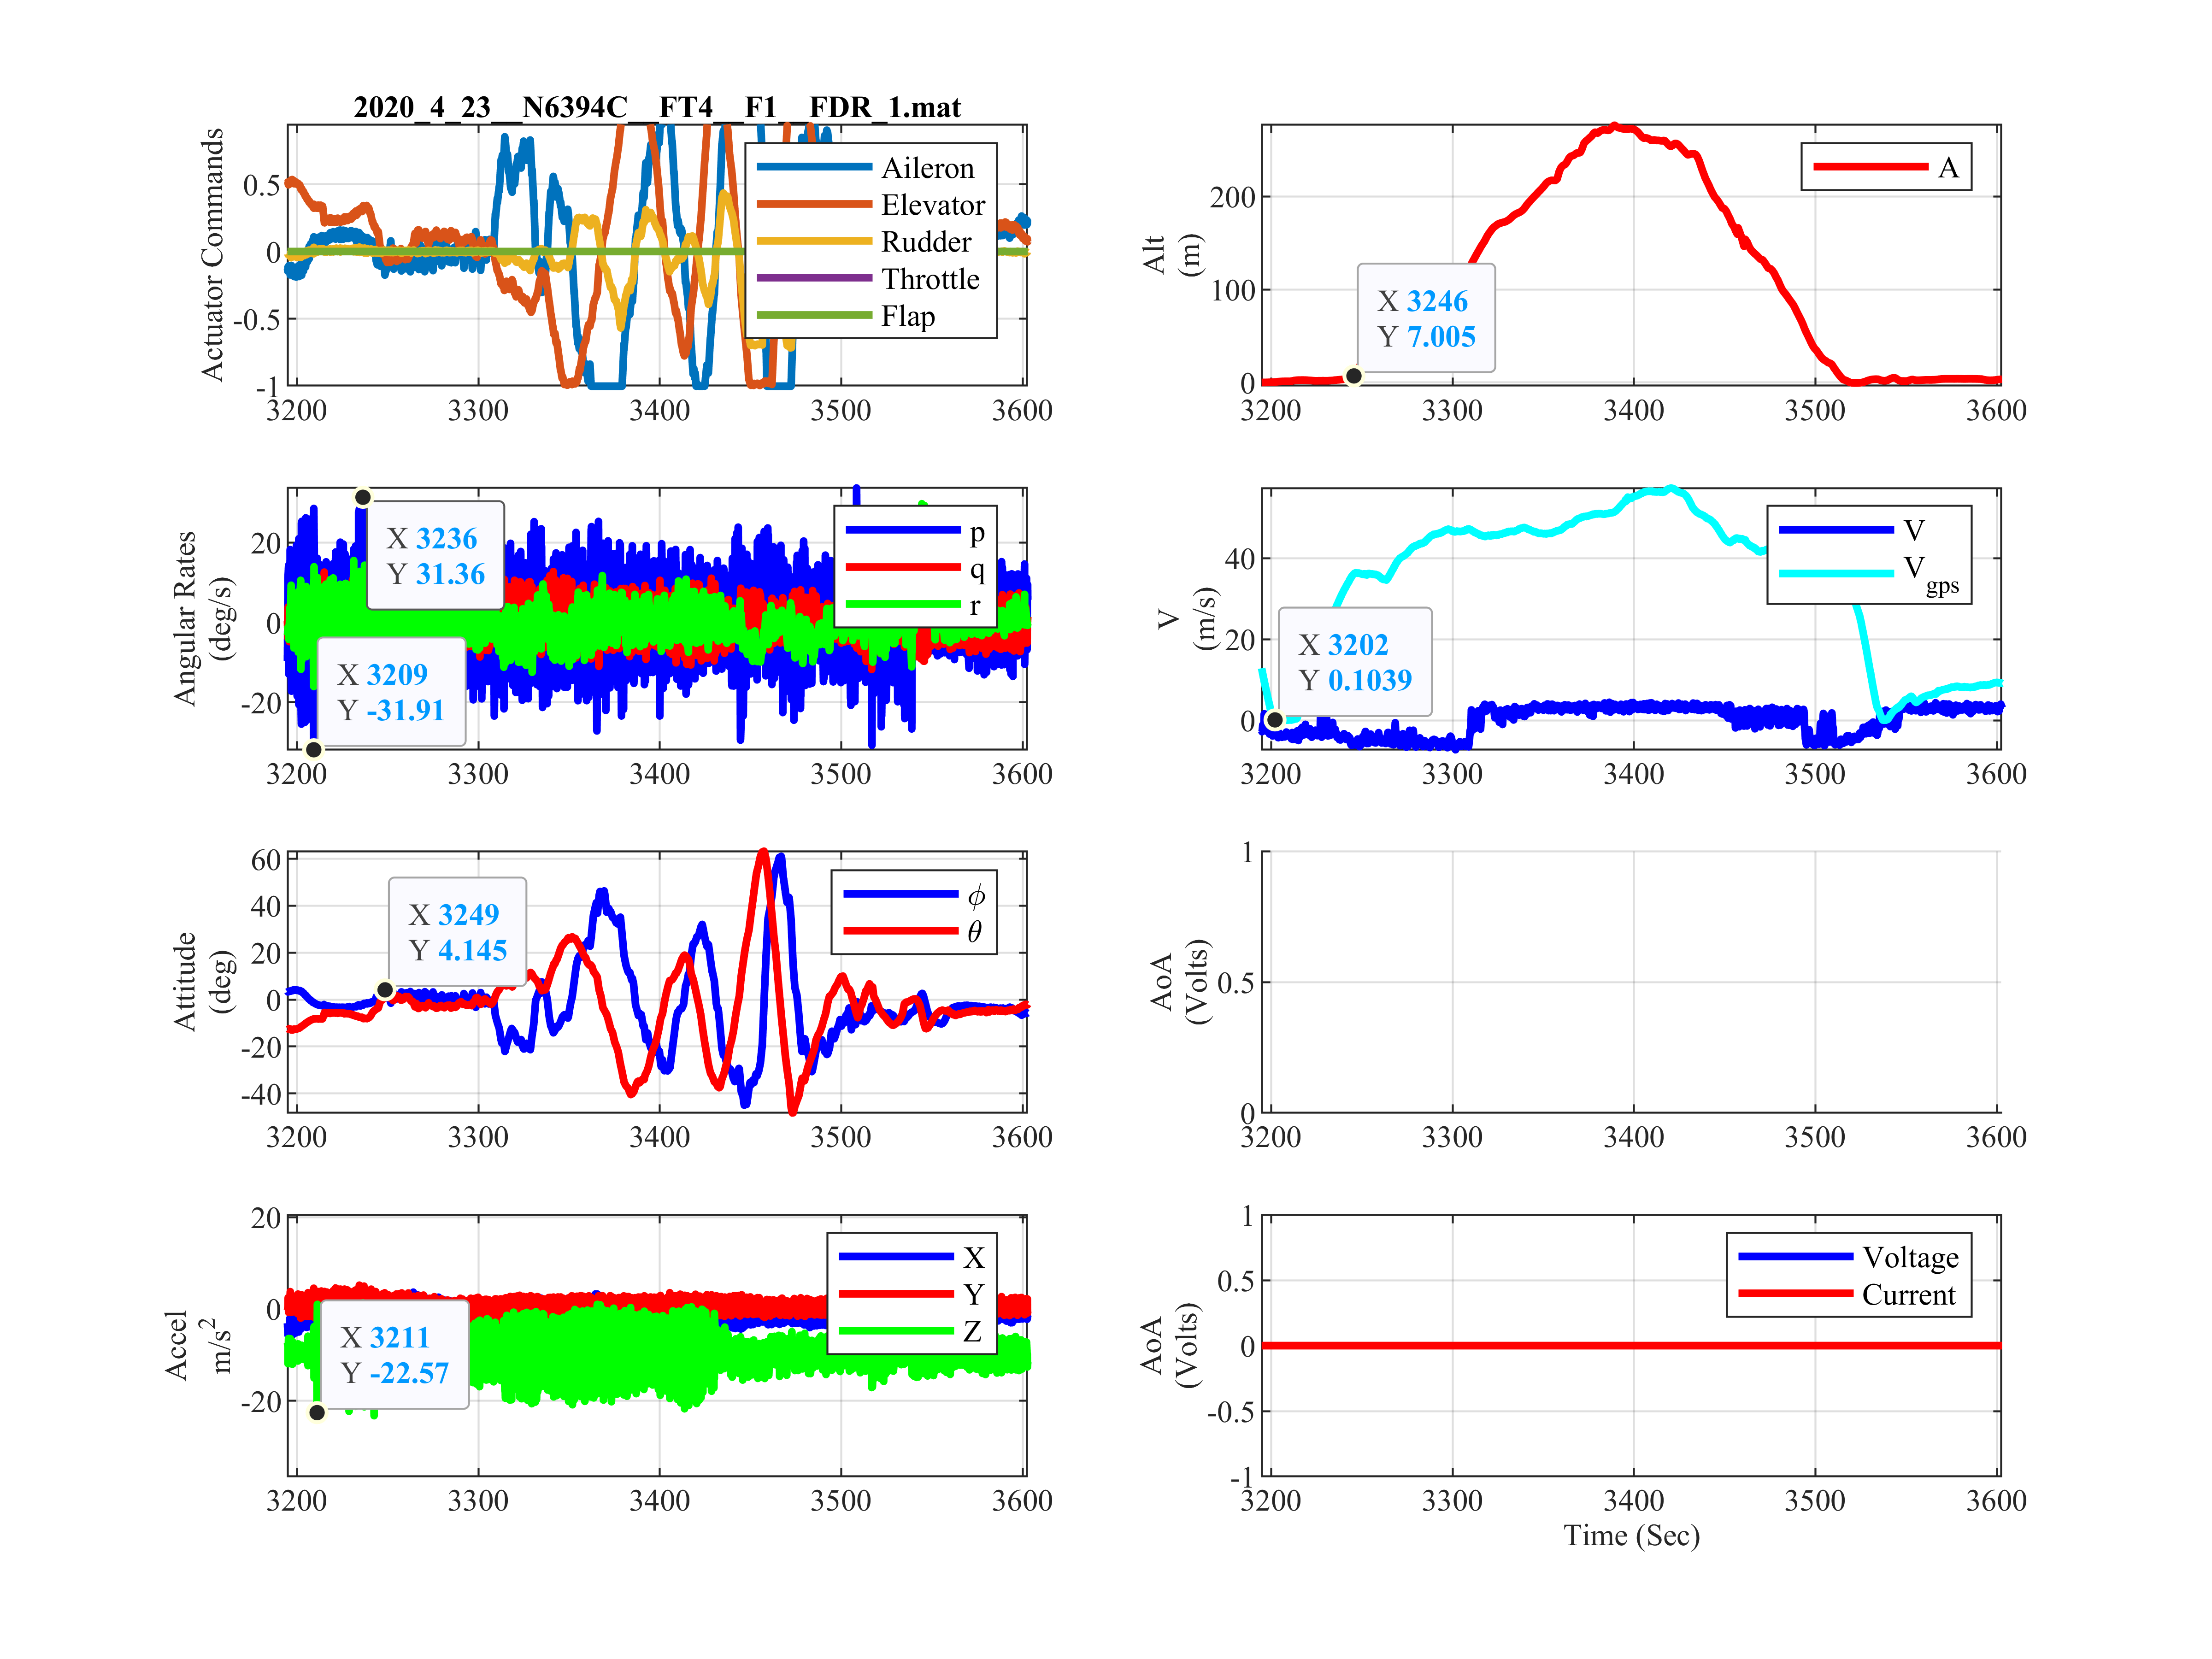
\includegraphics[height=4in]{LandingRollTimeID.png}
	\caption{Example of Identification of takeoff Roll Start and End Times.}
	\label{landingtimeid}
\end{figure}

\begin{figure}[htp!]
\centering
	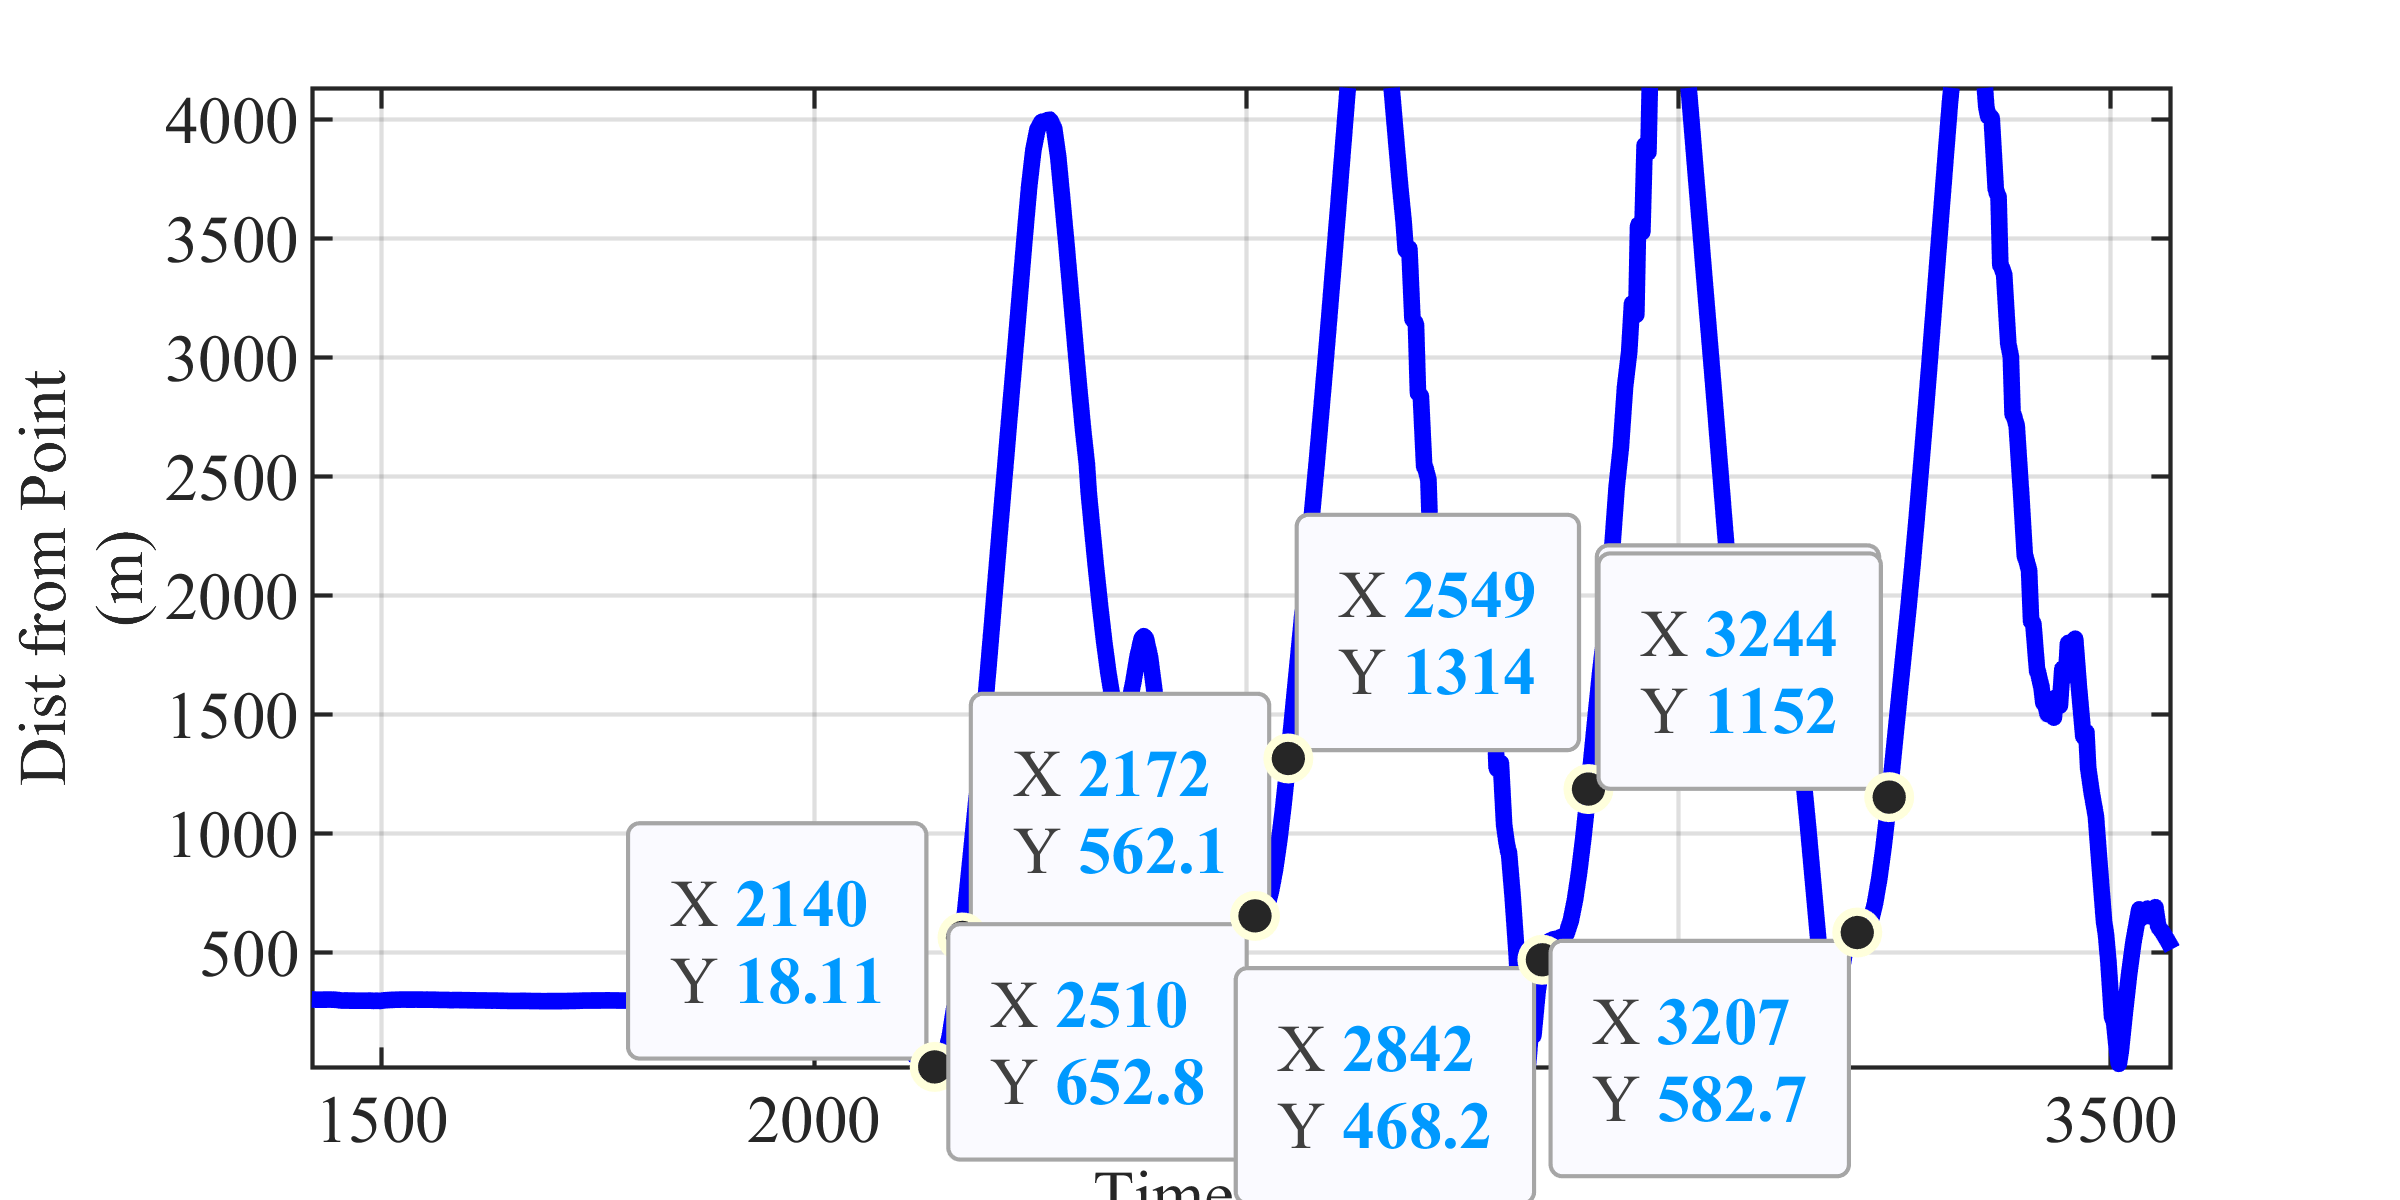
\includegraphics[height=2in]{LandingRollDistID.png}
	\caption{takeoff Roll Distance Identification using Previously Identified Time Instants.}
	\label{landingdistanceid}
\end{figure}

Assuming the same conditions as before, the POH specified landing roll is around~\SI{700}{\foot}.  The identified landing roll was around~\SI{1200}{\foot} which is nearly twice as long of a roll as predicted by the POH. This error is explained by a number of factors.

The first of these factors is that the airplane for the flight test was a rented airplane and as much as the pilot in this case has a history of tearing up rented vehicles, hammering the brakes on a rental airplane and causing damage to the landing struts, shredding the tires or burning up the brakes would be bad for a number of factors. Firstly, any of these events would have prevented further flight testing. Second, since the flight test was at the behest of the University, there could have been repercussions for repair costs incurred due to foolhardy piloting. Thus, to his credit, the pilot in this case may be blamed for being slightly cautious during the landing performance evaluation.  Since the pilot is more familiar with different aircraft types, it is also possible that he was not exercising the full performance of the aircraft simply due to lack of familiarity.

Additional factors must not be discounted. Namely, the load estimate used here is an estimate since fuel load was not given in the test card. It is possible the airplane was loaded more in reality than was accounted for here. Additionally, since this a rental airplane, presumably with many hours on the engine and many sloppy landings on the airframe, it is possible that the braking action is diminished. The tires could be worn to the point of decreasing available braking force. The hydraulic system could be improperly bled leading to spongy feel, fluid boiling and lack of brake force. The rotors and pads themselves could be worn out or of inferior quality which could all lead to diminished braking action.

The POH landing estimate is for a full stall landing. This means that the touchdown point at the end of the flare perfectly corresponds to the threshold minimum speed where the aircraft is no longer flying. It is highly unlikely that this condition is perfectly matched during flight. Undershooting landing speed at this critical condition would most likely lead to a crash. Whereas overshooting this critical speed simply leads to a longer landing roll. The conservative approach will always result in a longer landing roll out of the necessity to be safe. In this case, the pilot was aiming for a specific point on the runway during landing. This could also contribute to the longer roll since for true landing performance, the aircraft should be brought near the runway and flown nearly level just above the runway until the stall condition is approached and the aircraft touches down. In this case, more conventional landing technique was used meaning that the glide slope is an important factor in determining touch-down speed leading to changes in landing performance.

Additional problems are likely to be found with the way the roll length is estimated. For takeoff roll, the velocity estimate is fairly reliable since GPS gets better the longer  the vehicle is sitting still. For landing, since the aircraft is transitioning from high speed to low speed, the error in the GPS velocity estimate is likely higher. The data were cross referenced with data from other sensors; however, most noisy sensor rely on an estimate to get in the ballpark of the correct location. This has been previously discussed and it could mean that the start and end time estimates from cross-referenced sensors are simply confirming the estimate which has already been found.

The take-away here is that you should not expect to rent a Piper Warrior and go enter a short takeoff and landing (STOL) competition without first verifying that the short field takeoff and landing roll estimates are correct. This is not the correct airplane for bush flying anyway, but if your home airport is a~\SI{1000}{\foot} grass strip, then maybe you should look elsewhere. It is also possible that this aircraft has updated load information or some other mitigating factors explained in the POH which belongs to this aircraft. POH are customized according to modifications to the aircraft and updated throughout the life of the plane. It is possible that some factor (including those not mentioned above) has been documented in the POH and would explain the relatively poor landing roll performance.

\FloatBarrier

\subsection{Power Required for Level Flight}

The power required for level flight was identified by performing the maneuver previously described. This maneuver was identified on the internal data recorded using the measured GPS speed and barometric altitude. The start maneuver was identified by seeking the level altitude part of the flight. Once the start point was identified, the speed measurement was used to determine when the aircraft was at minimum power and then a maximum converged speed was identified after the speed increase due to the power increase during the maneuver.

Exhaustive time synchronization of the internal and external flight data recorders was outside the scope of this report. However, the external flight data recorded did contain airspeed information for this test. Since indicated airspeed (as measured by an air data probe) is the speed of interest for this flight test, the data was referenced. Rudimentary time synchronization was conducted simply by looking for the same altitude patterns in both internal and external files. Thus the time values doe not match perfectly; however, the data is still useful.

The comparison of the GPS recorded ground speed and the indicated airspeed in~\Cref{gpsspeedcomparison} suggest that this maneuver was conducted with a~\SIrange{5}{8}{\meter\per\second}. The minimum speed achieved during this flight test was~\SI{25.73}{\meter\per\second} (\SI{50.01}{\kts}) and the maximum speed achieved was~\SI{56.66}{\meter\per\second} (\SI{110.1}{knot}).

\begin{figure}[htp!]
\centering
	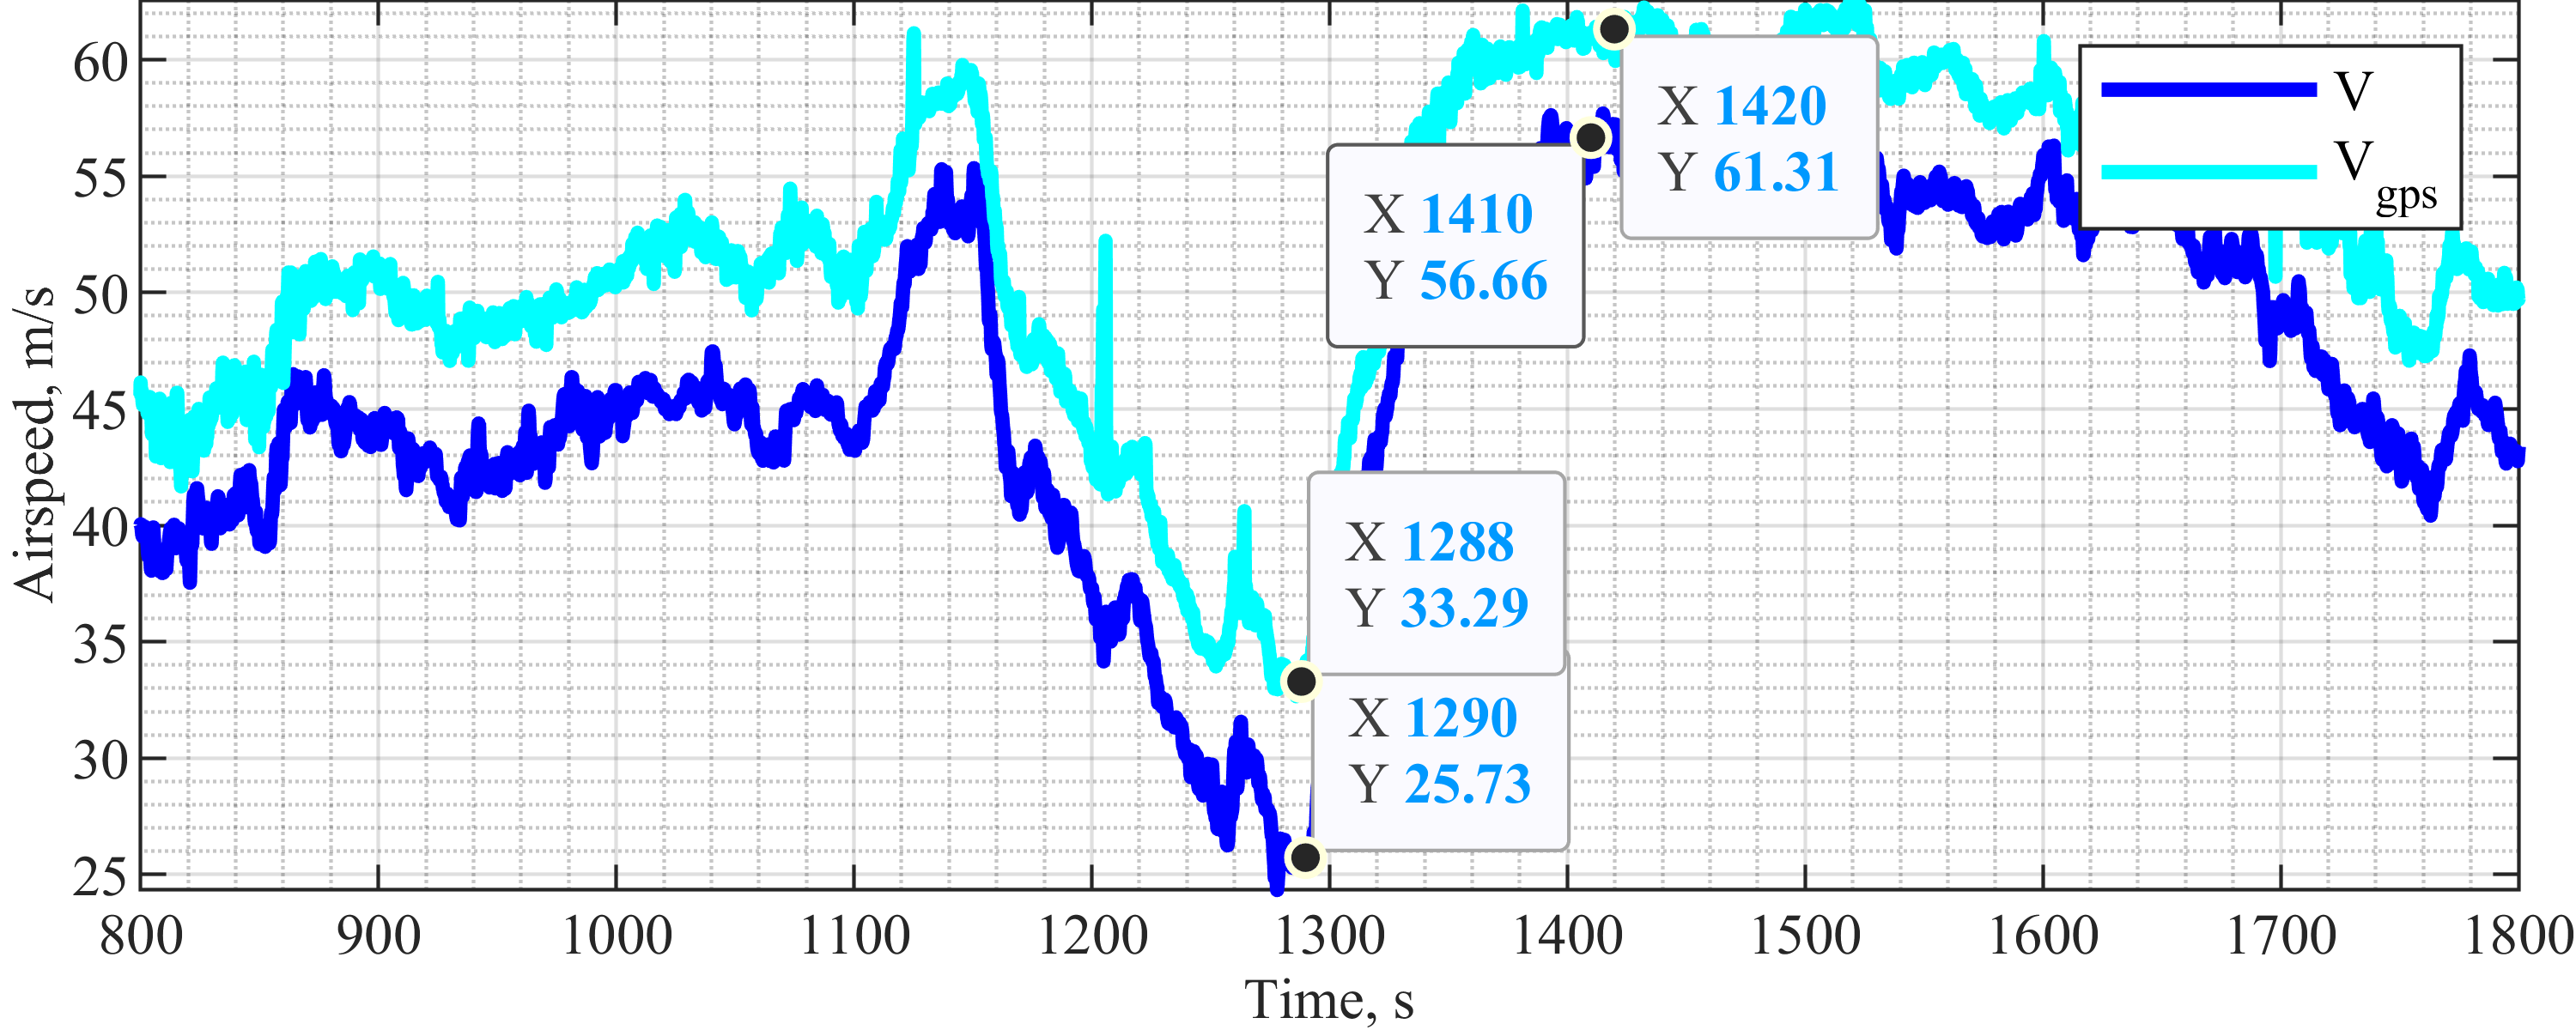
\includegraphics[height=2in]{GPSSpeedComparison.png}
	\caption{GPS Ground Speed vs. Indicated Airspeed.}
	\label{gpsspeedcomparison}
\end{figure}

The GPS speed is shown overlaid with the barometric altitude in~\Cref{levelflightmaneuver}. The field height at KMKC airport is approximately~\SI{750}{\foot} and the target altitude for this test was~\SI{3000}{\foot} AGL. This corresponds to an MSL altitude of approximately~\SI{1200}{\meter} so this the conditions for this test were not met precisely. Slight variation in target altitude should not have sufficiently affected the engine performance in order to influence these results. Provided the altitude was approximately constant throughout the test the results should be considered valid.

\begin{figure}[htp!]
\centering
	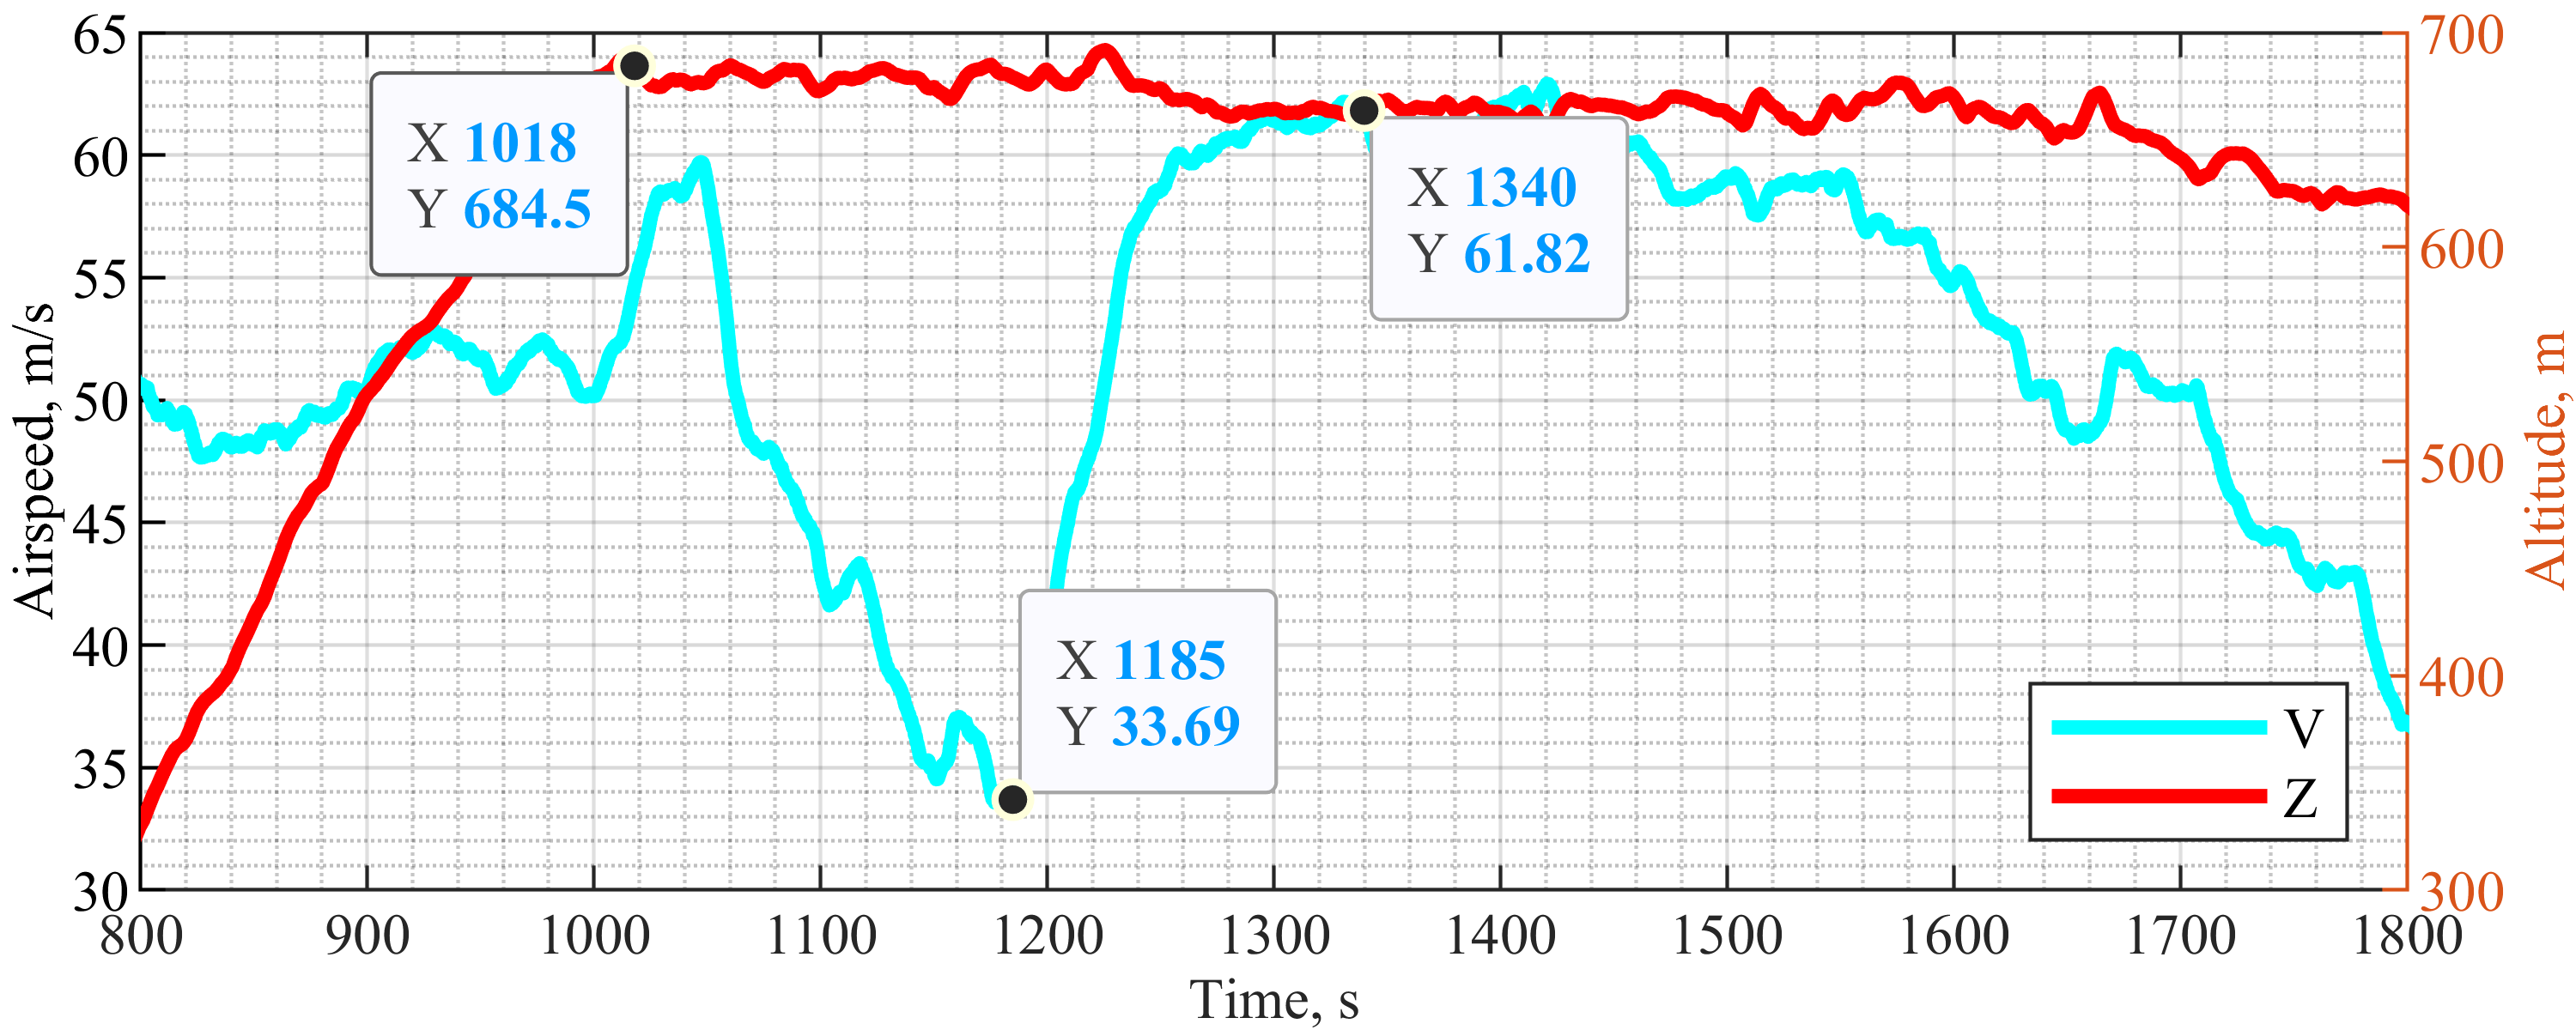
\includegraphics[height=2in]{LevelFlightPower.png}
	\caption{Level Flight Maneuver.}
	\label{levelflightmaneuver}
\end{figure}

In the clean configuration the Piper Warrior has a stall speed of~\SI{50}{\kts} and a maximum attainable speed of~\SI{126}{\kts}. The results of this flight test compare to the published capabilities very well. The tail wind could have had a slight effect on the results but the stall speed was within~\SI{6}{\kts} of the expected value (an error of around~\SI{10}{\percent}) and the maximum speed was within~\SI{16}{\kts} (an error again of slightly more than~\SI{10}{\percent}). The aircraft in its current configuration is most likely not as clean as the day it was manufactured and the engine has most likely lost some power. Thus the expected maximum speed would be lower than that published in the POH. Additionally, the dirtier aircraft may be subject to stall at a slightly higher speed. This is contrary to the understanding of flaps wherein a dirtier aerodynamic aircraft stalls at a lower speed but consider that flaps are an intentional modification which increase lift at the cost of increased drag. Increased airframe dirtiness due to aircraft skin defects, or dirt or panel misalignment, panel vibration etc. is an unplanned effect where drag is increased most likely with no corresponding increase in drag.

\FloatBarrier

\section{Discussion}

\begin{itemize}
	\item Power required for level flight
	\begin{itemize}
		\item Show power required vs. airspeed plot (individual points and regression, if appropriate)
		\item Identify minimum power required and corresponding airspeed
		\item Identify maximum range and corresponding airspeed
		\item Compare airspeed with published data
	\end{itemize}
	\item Climb performance
	\begin{itemize}
		\item Show climb rate vs. airspeed climb polar (individual points and regression, if appropriate)
		\item Identify maximum climb rate and corresponding airspeed
		\item Identify maximum climb angle and corresponding airspeed
		\item Compare airspeeds with published data
	\end{itemize}
	\item Gliding performance
	\begin{itemize}
		\item Show descent rate vs. airspeed glide polar (individual points and regression, if appropriate)
		\item Identify maximum sink rate and corresponding airspeed
		\item Identify best glide speed and corresponding airspeed
		\item Compare airspeeds with published data
	\end{itemize}
\end{itemize}

\section{Conclusions}

\begin{itemize}
	\item Summary of test objectives
	\item Summary of process
	\item Summary of findings
	\item Recommendations
\end{itemize}

Innocuous changes in another section.

\section{Appendix}

Dummy github changes.

\end{document}
